\chapter{Introduction}
\label{chap:introduction}
\graphicspath{01-Introduction/img}

\section{Motivation}
\label{sec:intro-motivation}
In early 2024, the world population was estimated at 8.X billion people and is expected to continue to grow, potentially reaching 9 billion and beyond by 2050 \citep{godfray_food_2010}. Just a year earlier, \cite{richardson_earth_2023} reported that six of nine so-called ``planetary boundaries'' of fundamental processes in the Earth system had been crossed, meaning that it is becoming increasingly difficult to ensure that our planet remains habitable and safe for all humans \citep{rockstrom_planetary_2009,rockstrom_safe_2023}. Thus, ensuring that a growing world population has equitable access to the amount of nutrients and calories required for a healthy diet, and lives in an intact environment in terms of clean air, water and biodiversity, is probably one of the greatest challenges facing humanity today.

Among the driving forces that have shaped our planet the most, agriculture plays a prominent role \citep{campbell_agriculture_2017,winkler_global_2021}. Not only has agriculture enabled the creation of permanent settlements, complex social structures and population growth, it has also altered the Earth's surface to such an extent that about one third of the Earth's land surface is covered by agricultural land, equivalent to about 48 million $km^2$. Of this area, according to \cite{faostat_faostat_2021}, 23\% or about 11 million $km^2$ was crop land in 2021, which is larger than the size of the USA (9.8 million $km^2$). Despite this huge area, a surprisingly small number of crops are grown on it, with cereals such as wheat, maize and rice accounting for 7.2 million $km^2$ (65\%) of the world's arable land and an estimated yield of around 2819 million $tons$ \citep{fao_fao_2023} in 2023. In other words: A significant part of our calorie intake depends on the ability of a few species from the \textsl{Poaceae} family to produce stable yields.

However, the ability of these crops to produce stable yields and keep pace with the projected growth in the world's population and changing dietary habits is challenged for a variety of reasons \citep{tilman_global_2011}. Human-induced climate change has multiple impacts on crop production, but overall there is consensus that the impacts on food security are potentially severe \citep{schmidhuber_global_2007,godfray_food_2010,rezaei_climate_2023}. Climate change is mainly driven by emissions of greenhouse gases such as carbon dioxide ($CO_2$) or methane ($CH_4$) \citep{ipcc_summary_2023}. While C3 crops such as wheat could potentially benefit from elevated $CO_2$ levels, increases in the productivity of these crops could be offset by the negative effects of more extreme heat and drought events, leading to projected yield losses of between 6 and 23\% \citep{rezaei_climate_2023}. Notably, up to a quarter of these emissions come from agricultural activities including ploughing, extensive use of fertilisers, livestock farming, or agricultural land-use changes such as deforestation or wetland drainage \citep{laborde_agricultural_2021}. In a changing climate, the incidence and geographical distribution of plant pathogens are also likely to pose new challenges to crop production \citep{burdon_climate_2020}. At the same time, agriculture is the largest consumer of water (70\% of global annual water demand), making it vulnerable to the effects of prolonged droughts \citep{meza_global-scale_2020}, and subject to economic conflicts over the allocation of scarce water resources \citep{rosa_global_2020}. In addition, recent evidence suggests that crop water use efficiency has stagnated since 2001, most likely due to increases in vapour pressure and evapotranspiration, posing further challenges to maintaining agricultural production levels \citep{li_global_2023}. In addition to the effects of climate change, issues related to soil degradation \citep{bindraban_assessing_2012}, biodiversity loss \citep{lanz_expansion_2018, abdi_biodiversity_2021} and the effects of run-off from fertilisers and pesticides -- which have contributed significantly to past increases in agricultural productivity \citep{pingali_green_2012} -- should be mentioned.

Given these challenges, and the need to increase global food production by up to 70\% to meet the demands of a growing world population \citep{hertel_global_2011} while remaining within planetary boundaries, it is clear that crop production must become more resource-use efficient, less polluting and more resilient to hazardous events using existing arable land and soil resources. Increasing the resilience and resource efficiency of crop production can be achieved in two ways:

One is to adapt farming practices. This includes precision agriculture, i.e. the application of fertilisers, growth regulators and pesticides at the right time, in the right place and in the right quantity \citep{finger_precision_2019}, no-tillage systems \citep{triplett_notillage_2008} or measures to increase the diversity of species grown on a parcel, such as strip cropping \citep{juventia_spatio-temporal_2022} or variety mixtures (paper flavian).

The second pathway is related to the crops themselves. For example, breeding varieties that escape abiotic stressors through an accelerated development cycle could reduce the risks of extreme heat associated with climate change \citep{rezaei_climate_2018, rogger_can_2021}. At the same time, the rather slow process of variety breeding needs to be accelerated to keep pace with the rate of environmental change \citep{zhang_climate_2022}, using innovative approaches such as physiological breeding \citep{reynolds_physiological_2016} and genomic prediction \citep{desta_genomic_2014}. Both pathways are arguably interlinked and require solid knowledge of crops, their growth and development cycles to make well-informed decisions.

The main motivation for this work is to study crops such as wheat in their environment, i.e. in the interplay of anthropogenic and natural factors, in order to enable well-informed decisions. Bearing in mind the vast area on which cereals such as wheat are grown worldwide, the method should be able to provide large area coverage up to global scale without exceeding the budget of agricultural researchers in the field, who are at the heart of the required transformation process. At the same time, given the short-term nature of many environmental processes, the method should provide relatively high temporal resolution (up to days). Most importantly, the method should provide results that can be used directly in the decision-making process, and that are both interpretable and traceable. Among the many facets of crop production, the focus of this work is on the growth and development of winter wheat (\textsl{Triticum aestivum}), which had an estimated annual production of 819 million $tons$ in 2023 (29\% of the total world cereal yield), grown on an area of about 2.2 million $km^2$ (20\% of the world arable land).

\section{Theoretical background}
\subsection{Plant growth and development}
\label{subsec:intro-plant-growth-dev}

Growth and development are essential terms for describing the life cycle, form and functioning of plants, which is the subject of physiological research \citep{leopold_plant_1964}. Here we define growth as the increase in the number of cells in a plant tissue and development as the appearance of new plant structures or organs such as buds, roots, shoots and leaves. The formation of new cells is driven by tissues of high mitotic activity called apical meristems \citep{sinnott_growth_1939}. The apical meristem consists of undifferentiated stem cells \citep{bowman_formation_2000}, i.e. cells that have the ability to take on almost any other cell form (totipotency). While differentiated plant cells cannot normally divide, meristematic cells can continue to divide until they themselves become differentiated. Therefore, most of the increase in the number of cells in a plant comes from meristematic cells in the shoot apical meristem (above ground part of the plant) and in the root meristems (below ground) \citep{kerstetter_shoot_1997}.

To better understand the intuitive meaning of growth and development, an illustrative example on a single leaf and a single plant is given in Figure \ref{fig:growth-development-biology}. In figure \ref{fig:growth-development-biology} on the left, growth refers to the increase in size and weight of a plant leaf as a result of continued cell division in the shoot apical meristem. Traits such as leaf area, leaf length or dry matter, i.e. the dry weight of the leaf, allow growth to be quantified. At the same time, the apical meristem is responsible for the formation of new leaves - a process called development (Figure \ref{fig:growth-development-biology}, right). A developmental trait is, for example, the number of leaves on a stem.

It is clear, therefore, that plant growth and development are linked and rely on the same underlying biological mechanism of cell division and differentiation. Furthermore, growth and development are processes that are a function of time \citep{prusinkiewicz_modeling_2004}. The term phenology describes the timing of different stages of plant development, such as germination or the onset of flowering \citep{piao_plant_2019}. In the example from Figure \ref{fig:growth-development-biology}, a phenological stage of development is the appearance of a new leaf. Scales such as \gls{BBCH} have therefore been defined to allow unambiguous communication of development between plant scientists or to agricultural practitioners \citep{lancashire_uniform_1991}.

The rate of growth and development depends on the levels of plant hormones \citep{shani_role_2006}. Although hormone levels can also be controlled by synthetic plant growth regulators \citep{gaspar_plant_1996}, external environmental covariates such as photoperiod, temperature \citep{porter_temperatures_1999}, \gls{PAR} \citep{abbate_effects_1995} and the availability of resources such as nutrients and water control a considerable proportion of growth and development rates \citep{masle_competition_1985,korner_paradigm_2015}.

\begin{figure}[H]
    \centering
    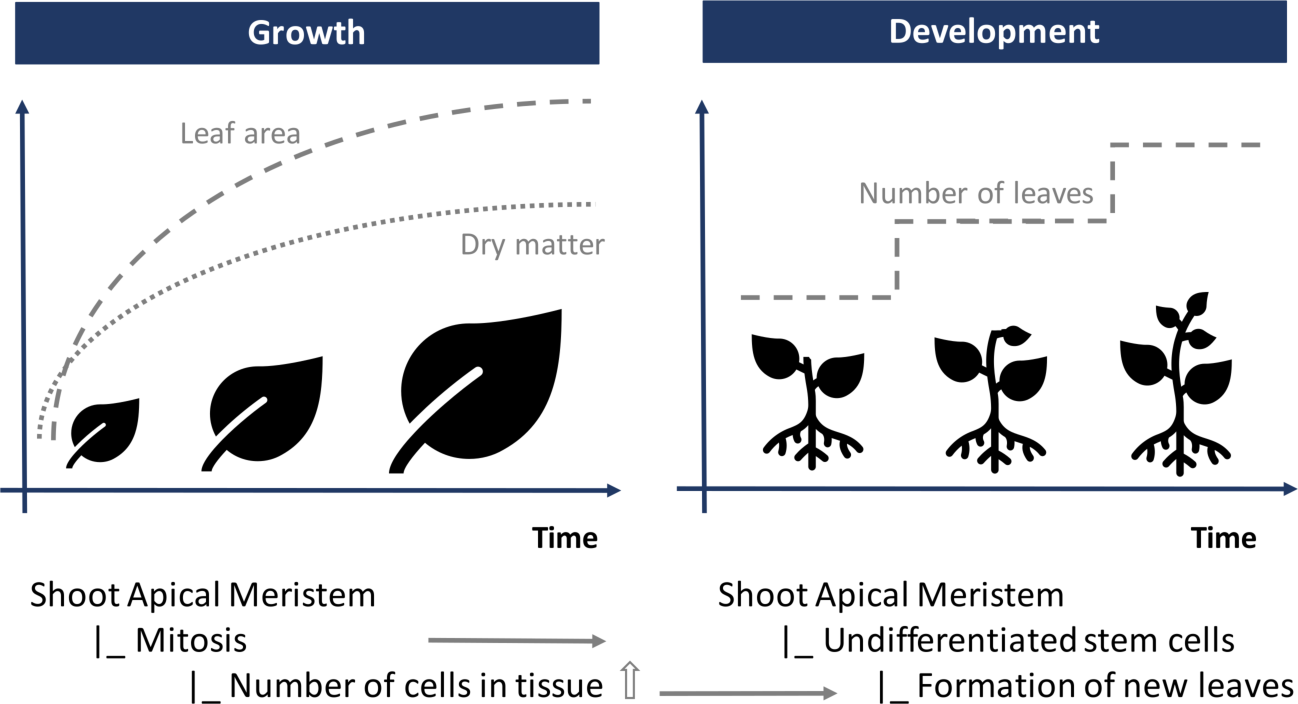
\includegraphics[width=\textwidth]{01-Introduction/img/growth_and_development.pdf}
    \caption{Illustrative example of leaf growth (left) by means of increasing leaf size and weight and plant development (right) by means of the appearance of new leaves from the main stem.}
    \label{fig:growth-development-biology}
\end{figure}

\subsection{Growth and development in winter wheat}
\subsubsection{Qualitative assessment}
\label{subsubsec:ww-qualitative-assessment}

Winter wheat is an annual crop that uses the C3 photosynthetic pathway to fix atmospheric carbon. In the northern hemisphere, winter wheat is sown in the autumn (September to November in central Europe) and harvested in the summer (June to August) of the following year. Like all flowering plants, the development of winter wheat can be divided into a vegetative and a reproductive phase. To trigger this transition, winter wheat requires vernalisation during the winter dormancy \citep{fedorov_photoperiodism_1976}, i.e. exposure to cold temperatures for a prolonged period.

Based on a growth perspective, \cite{kirby_analysis_1988} proposed to divide the growth and development process into three phases: The first \gls{GS}, \gls{GS} 1, consists of the formation of leaves and spikelets from the shoot apex. After leaf development, tillers emerge from the leaf axils. \gls{GS} 1 continues until the formation of the terminal spikelet. \gls{GS} 1 is followed by vertical elongation of the stem and the spikelet in \gls{GS} 2, the so-called \gls{SE} period. \gls{GS} 2 ends with the onset of anthesis, i.e. when the inflorescence has fully emerged from the flag leaf sheath. In the third and final stage, \gls{GS} 3, growth and development are mainly restricted to grain formation, filling and ripening, and the plant reaches physiological maturity with the completion of senescence. Here, carbon assimilation stops and nitrogen-rich plant pigments such as chlorophyll in the leaves, no longer needed for photosynthesis, are gradually broken down and converted into proteins to fill the grain \citep{thomas_stay-green_2014}. Visually, this results in a ``browning'' of the canopy.

Figure \ref{fig:ww-growth-qualitative} shows images of winter wheat canopies between \gls{GS} 1 and 3. The individual \gls{GS} have been further subdivided into more fine-grained developmental stages, from leaf emergence to physiological maturity, and labelled with the corresponding \gls{BBCH} stages, to allow a clear description and communication of crop phenology \citep{lancashire_uniform_1991}. In Figure \ref{fig:ww-growth-qualitative}, there is a clear transition from low ground cover at \gls{GS} 1 (leaf development and tillering) to maximum ground cover at \gls{GS} 2 in the booting phase. In the heading stage, the inflorescence gradually becomes visible and is fully emerged before anthesis in \gls{GS} 3. With fruit development and ripening, grain filling begins, which is accompanied by senescence of the plant. Senescence begins in the lowest leaf layers and finally reaches the flag leaf, at which point the plant -- consisting entirely of non-photosynthetically active biomass -- has reached physiological maturity. In addition, Figure \ref{fig:ww-growth-qualitative} shows the typical timing in relation to phenology of management practices such as nitrogen fertilisation and the potential occurrence of biotic -- such as powdery mildew -- and abiotic stressors -- such as frost damage.

Building on the three phases proposed by \cite{kirby_analysis_1988}, the focus of this work was on winter growth and development in late \gls{GS} 1 and full \gls{GS} 2, i.e. between tillering and full emergence of the inflorescence, which is predominantly the \gls{SE} period. \gls{SE} was chosen because of the importance of this period for grain yield development: \gls{SE} marks the transition from vegetative growth in the tillering phase (\gls{GS} 1) to reproductive growth. Specifically, the shoot apical meristem (see Section \ref{subsec:intro-plant-growth-dev} and Figure \ref{fig:growth-development-biology}) switches from leaf formation to the production of spikelets and the initialisation of florets on the spikelets \citep{mcmaster_simulating_1992}. The duration and environmental conditions during \gls{SE} thus contribute to the number of fertile florets through successful meiosis \citep{villegas_daylength_2016} and the partitioning of biomass to the spikelets \citep{gonzalez_grain_2003}. Therefore, \gls{SE} is important for the final grain yield \citep{fischer_yield_1975,fischer_wheat_2011}.

Moreover, Figure \ref{fig:ww-growth-qualitative} highlights that \gls{SE} is important not only for grain yield formation but also in terms of agricultural practice, as the period studied in this work from tillering to anthesis overlaps with the optimum timing of the three nitrogen fertiliser applications \citep{lewis_effect_1938} and the potential occurrence of stresses (Figure \ref{fig:ww-growth-qualitative}, middle and bottom row).

\begin{figure}[H]
    \centering
    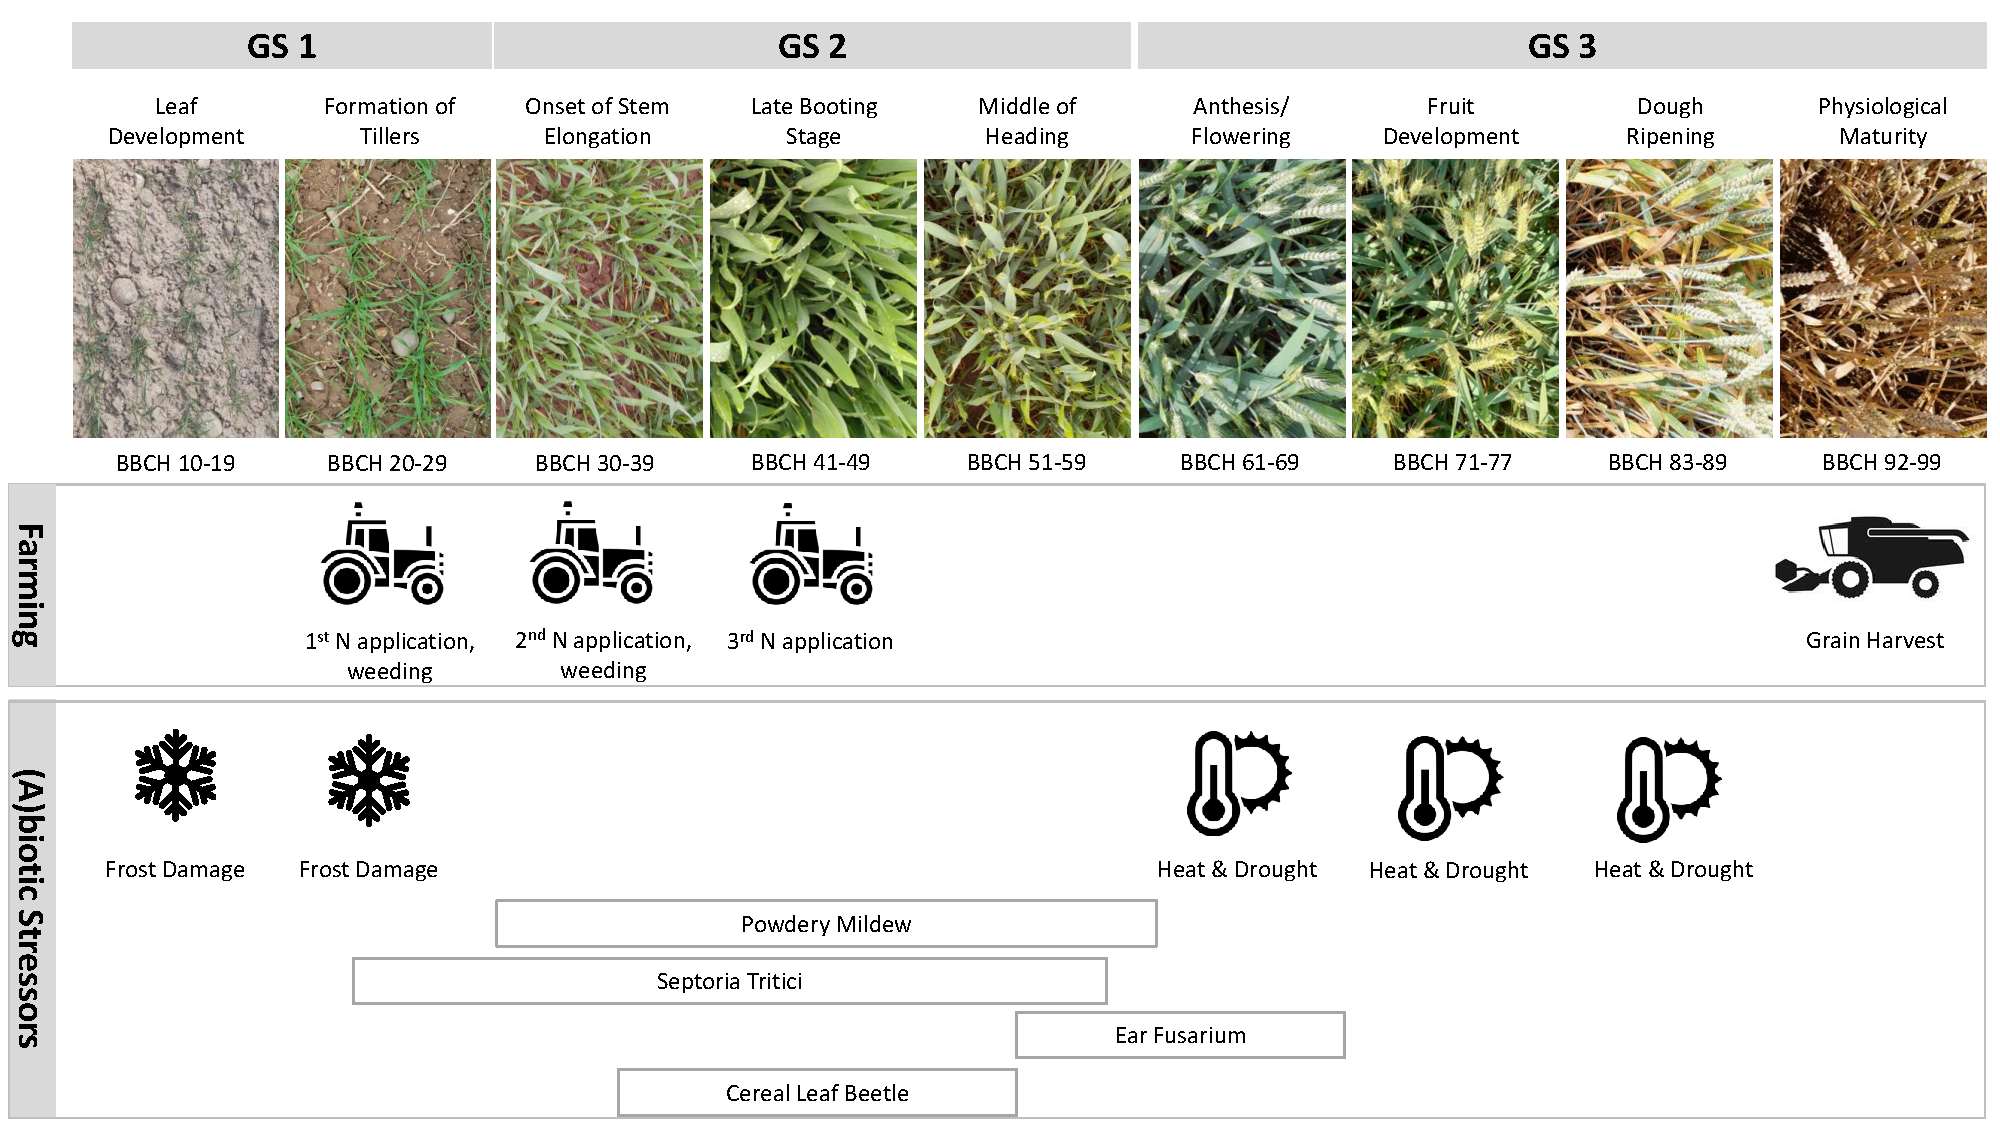
\includegraphics[width=\textwidth]{01-Introduction/img/wheat_developement.pdf}
    \caption{Qualitative overview about growth and development in winter wheat between grow stages (GS) 1 and 3 showing images of winter wheat canopies in different phenological development stages (expressed as \gls{BBCH} stages). In addition, the typical timing of important farming measures and occurrence of common abiotic and biotic stressors is shown.}
    \label{fig:ww-growth-qualitative}
\end{figure}

\subsubsection{Quantitative assessment}
On a macroscopic scale, as proposed in this thesis, the qualitative assessment of winter growth and development during \gls{GS} 1 and 2 outlined in section \ref{subsubsec:ww-qualitative-assessment}, can be quantified -- among other traits such as canopy height \citep[for example]{kronenberg_monitoring_2017} -- by increases (or decreases) in photosynthetically active, i.e. green, leaf area and above-ground dry matter, hereafter referred to as above-ground biomass.

Instead of leaf area, \gls{GLAI} is often used. \gls{GLAI} is defined as the one-sided photosynthetically active leaf area per unit of ground area \citep{watson_dependence_1958,maddonni_leaf_1996} and is therefore a proxy for photosynthetic capacity and hence productivity \citep{gitelson_productivity_2015}. Above-ground biomass quantifies the dry weight of all above-ground plant parts including not only leaves but also stems and grains. While in \gls{GS} 1 and 2, green leaf area and biomass are highly correlated \citep{aase_relationship_1978}, the partitioning of biomass into the grain by physiological maturity determines grain yield at harvest \citep{singh_harvest_1971}. In \gls{GS} 3, as noted above, the decomposition of chlorophyll into proteins leads to a decrease in \gls{GLAI} and an increase in the fraction of non-photosynthetically active biomass.

Figure \ref{fig:ww-growth-development} shows the temporal evolution of \gls{GLAI} in $m^2$ $m^{-2}$ (Figure \ref{fig:ww-growth-development}a) and above-ground biomass in $kg$ $ha^{-1}$ (Figure \ref{fig:ww-growth-development}b) in winter wheat with thermal time based on in situ data collected in 2022 and 2023 in Switzerland during this thesis. Thermal time -- also known as \gls{GDD} -- is defined as the accumulated daily mean air temperature in $^{\circ} C$ from the date of sowing above a base temperature of 0$^{\circ} C$ \citep{mcmaster_growing_1997}.

The \textsl{S}-shaped trajectory of \gls{GLAI} (Figure \ref{fig:ww-growth-development}a) during \gls{GS} 1 and 2 can be described by a logistic (aka sigmoid) model. \gls{GLAI} is mostly below 1 $m^2$ $m^{-2}$ during \gls{GS} 1 and increases to maximum values between about 4 and 7 $m^2$ $m^{-2}$ in \gls{GS} 2. With the onset of \gls{GS} 3 and senescence, \gls{GLAI} is expected to decrease towards values of $\sim 0$ $m^2$ $m^{-2}$ until physiological maturity is reached. Senescence and the corresponding decrease in leaf chlorophyll and hence \gls{GLAI} is not shown here, as this period was not the focus of this work.

Dry biomass (Figure \ref{fig:ww-growth-development}b) shows a monotonous increase from \gls{GS} 1 to \gls{GS} 3 from values around $\le$ 1000 $kg$ $ha^{-1}$ up to 10'000 $kg$ $ha^{-1}$ in \gls{GS} 3. In contrast to \gls{GLAI}, biomass values do not decrease during \gls{GS} 3 and can reach up to 20'000 $kg$ $ha^{-1}$ at physiological maturity. At the beginning of \gls{GS} 1, the biomass is almost entirely green leaf biomass. With tillering and stem elongation, the relative proportion of stem biomass increases (\gls{GS} 2). As the grain forms and fills in \gls{GS} 3, the green leaf biomass decreases and the grain biomass increases. Up to 50\% of the biomass at physiological maturity can then be allocated to the grain \citep{long_meeting_2015}.

\begin{figure}[H]
    \centering
    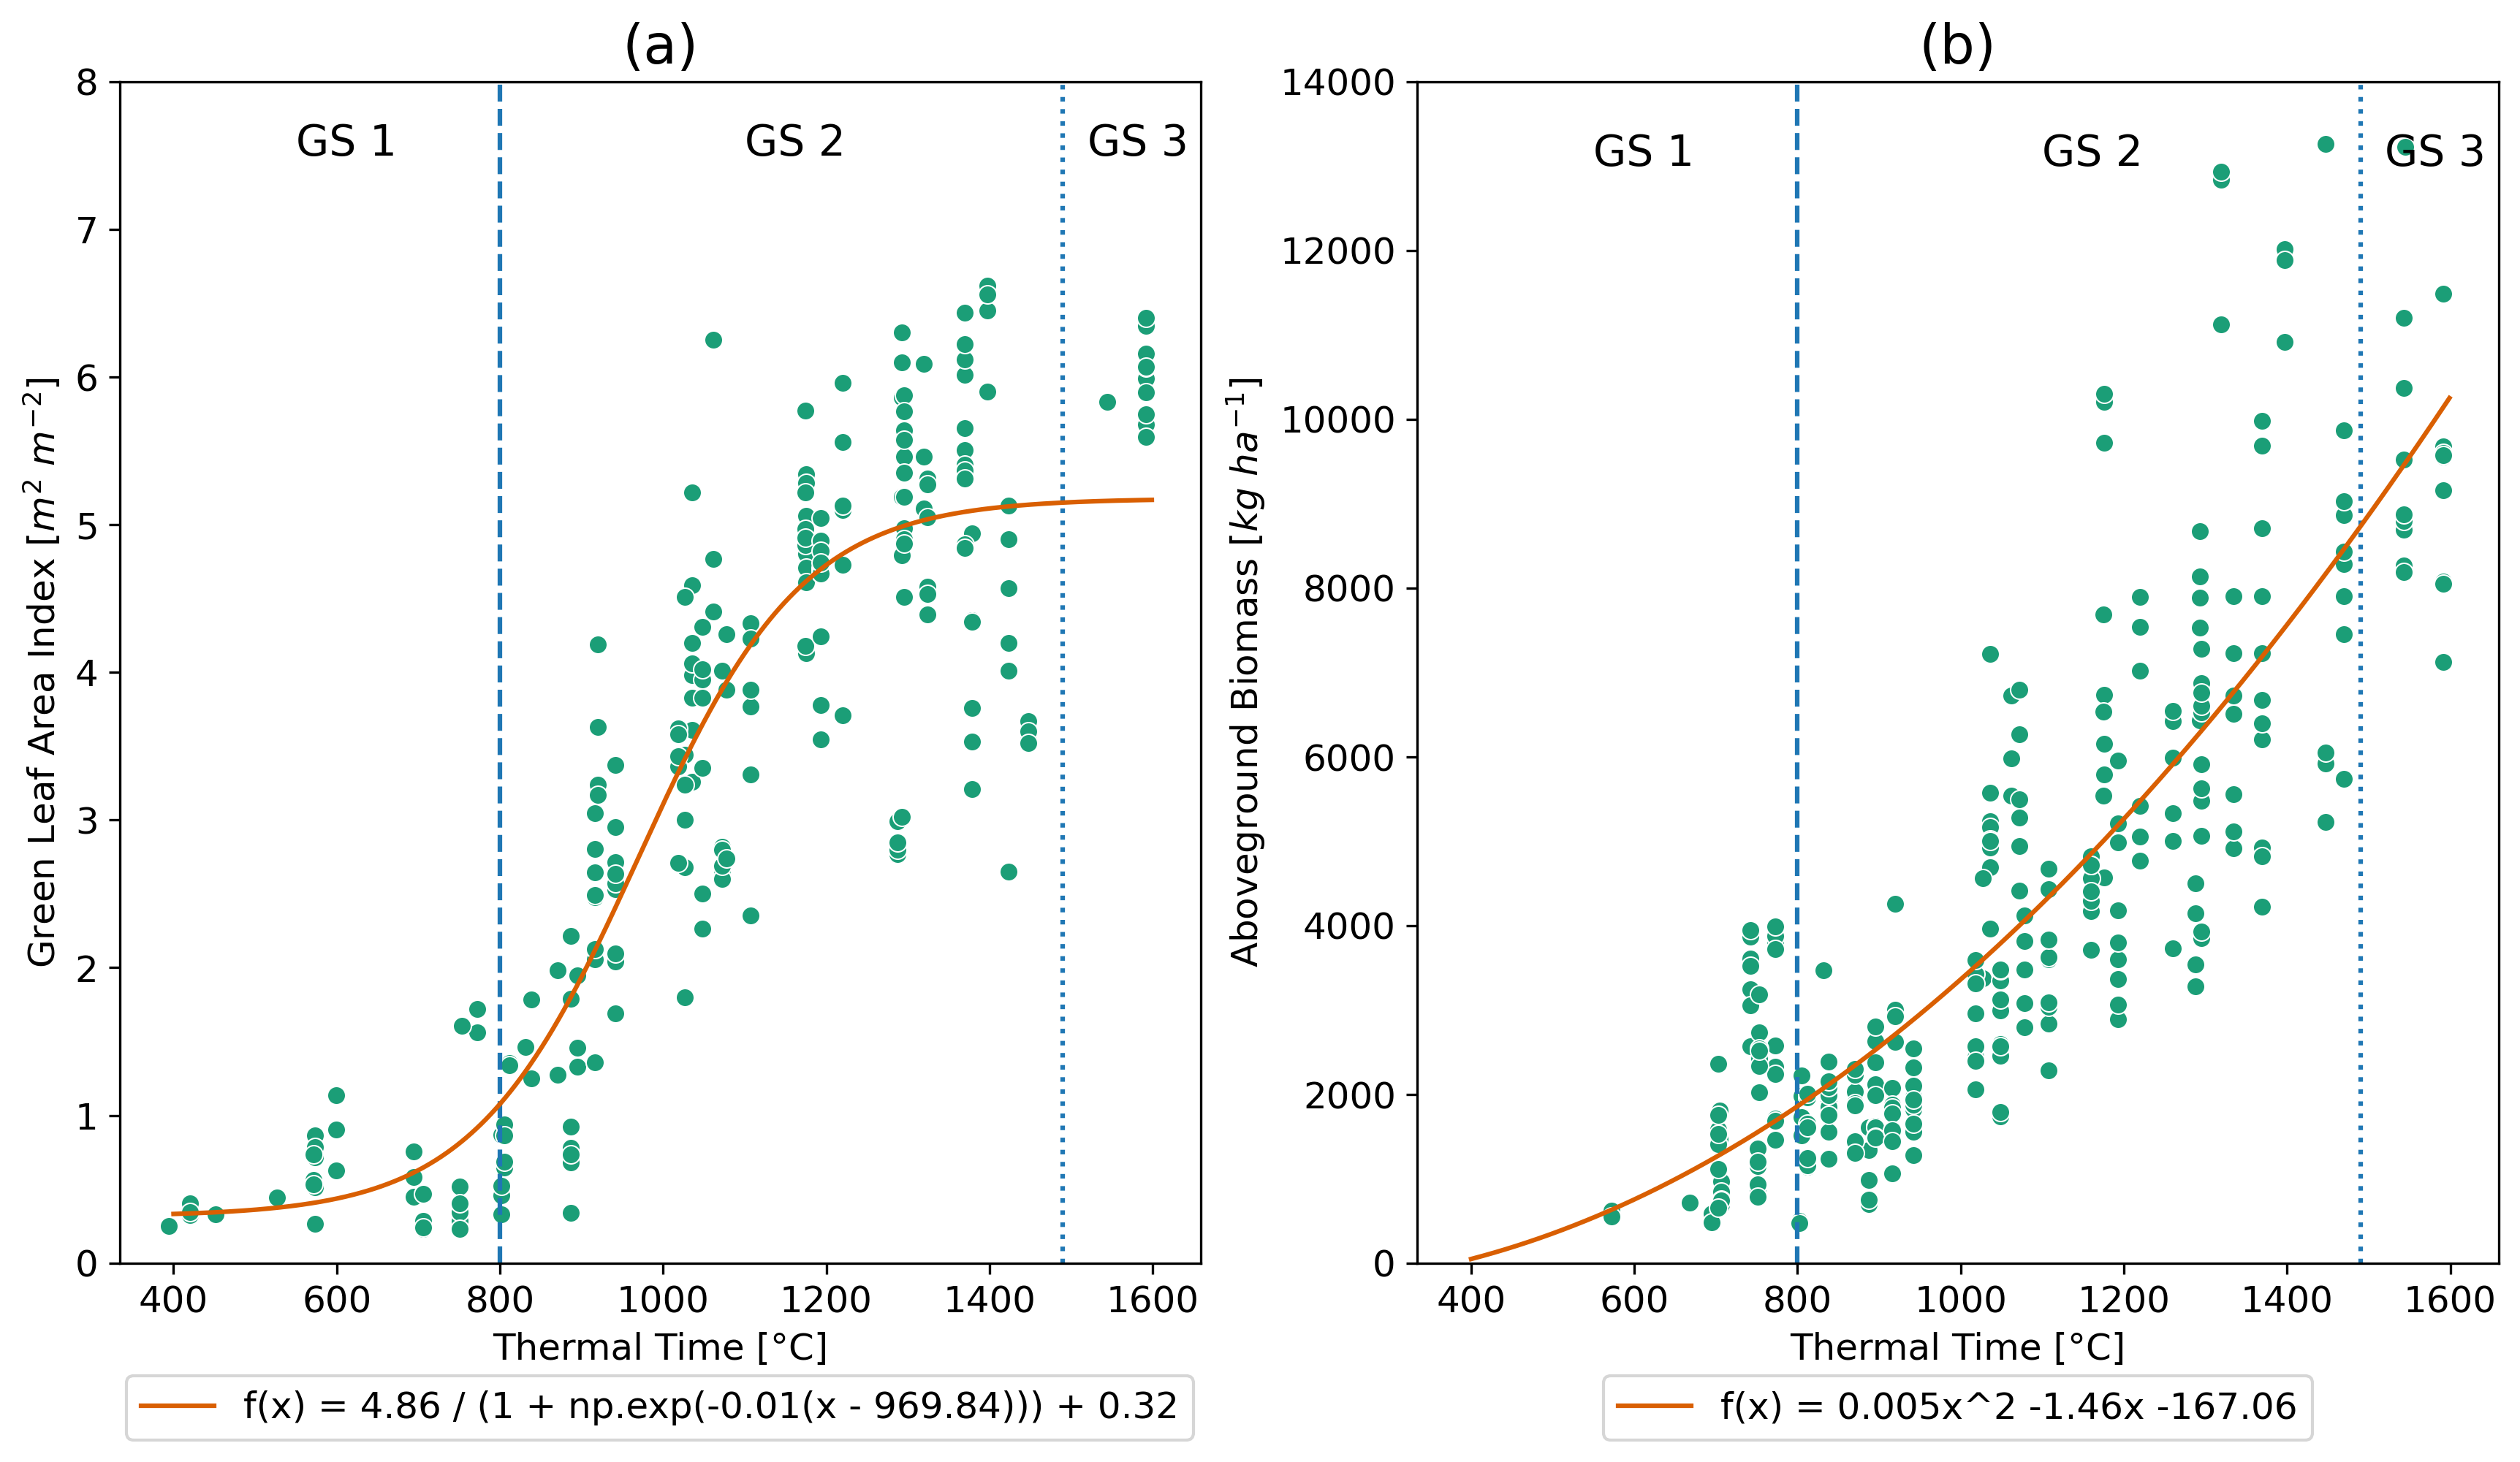
\includegraphics[width=\textwidth]{01-Introduction/img/glai_and_biomass_growth-stages.png}
    \caption{Temporal evolution of green leaf area index (a) and above-ground biomass (b) in winter wheat with thermal time, based on in-situ samples collected in 2022 and 2023 in Switzerland as part of this work. The growth stages (GS) proposed by \cite{kirby_analysis_1988} are separated by a dashed and a dotted line, respectively.}
    \label{fig:ww-growth-development}
\end{figure}

\subsection{Field phenotyping, remote sensing of vegetation, and earth observation}
\label{subsec:field-phenotyping-rs-eo}

Two disciplines have evolved to study plants and their interaction with the environment to provide quantitative estimates of plant growth and development: field phenotyping and remote sensing of vegetation.

\subsubsection{Field phenotyping}
\label{subsubsec:intro-field-phenotyping}
\paragraph{Definitions and principles}
Field phenotyping is the study of the functioning, development and biophysical and chemical properties of plants under field conditions \citep{walter_plant_2015} to provide a quantitative characterisation of their phenotypes. The phenotype is formed by the physical and thus observable characteristics of a plant as a result of interactions between the genome (G) and the environment (E) (G $\times$ E) \citep{johannsen_genotype_1911}. Traditionally, field phenotyping therefore aims to study G $\times$ E interactions -- sometimes including management (M) interventions such as fertilisation schedules \citep[for example]{rodene_uavbased_2022} -- to develop an understanding of the underlying physiological processes \citep{york_functional_2019}, poly-genetic control of traits \citep[for example]{singh_high-throughput_2019}, or to help select breeding lines \citep{pask_physiological_2012,roth_image-based_2023}.

This means that crop traits are recorded together with environmental covariates such as weather data. However, to study these interactions, spatial effects often need to be removed through statistical modelling \citep{piepho_twodimensional_2022}, as the number of replicates in terms of genotypes (varieties) and/or management systems required limits the number of effects that can be studied \citep{poorter_plant_1996}. 

Field phenotyping efforts are therefore typically limited to small spatial scales such as variety-testing trials, but provide a rich set of tools and knowledge from a plant physiological perspective on growth and development, which aligns with the motivation of this thesis.

\paragraph{State-of-the-art applications}
State-of-the-art field phenotyping is mainly carried out using mobile or stationary phenotyping equipment that allows the measurement of complex shoot and canopy traits throughout the growing season. Examples of such equipment include stationary, cable-suspended camera systems for repeated close-range imaging of hundreds of genotypes, such as the ``FIP'' field phenotyping platform operated by ETH Zurich \citep{kirchgessner_eth_2017}, or mobile phenotyping devices mounted on portable units \citep{crain_development_2016}, drones \citep{walter_advances_2022}, and field robots \citep{xu_review_2022}.

As noted above, a primary objective is to assist breeders by developing novel traits that allow earlier or improved selection of promising breeding lines \cite{watt_phenotyping_2020} and by characterising ``ideotypes'' \citep{roth_high-throughput_2022}. An ideotype represents an idealised, optimal genotype for a given environment \citep{donald_breeding_1968}. In response to the rapid progress in molecular biology and genome sequencing techniques, \gls{HTP} methods have emerged to overcome the so-called ``phenotyping bottleneck'', i.e. the characterisation of phenotypes has often not kept pace with the progress on the genotype side in recent decades \citep{araus_translating_2018, yang_crop_2020, song_high-throughput_2021}. \gls{HTP} methods have thus paved the way for the big data era in field phenotyping, with the acquisition of high-dimensional data on the whole phenotype, also known as (plant) ``phenomics''. \citep{houle_phenomics_2010}.

In particular, \gls{HTP} methods often resemble remote sensing methods, as many \gls{HTP} platforms are based on imaging sensors or ranging devices: Examples include the use of terrestrial laser scanners \citep{kronenberg_monitoring_2017} to estimate canopy height; multi-view optical imagery \citep{roth_extracting_2018} to approximate leaf area index; RGB images taken in nadir view to quantify canopy dynamics \citep{yu_image_2017}; pole-mounted RGB cameras (``phenocams'') to quantify growth and phenological development \citep{aasen_phenocams_2020}; thermal images from drones to quantify stomatal conductance \citep{perich_assessment_2020}; handheld hyperspectral spectroscopy to study senescence dynamics \citep{anderegg_spectral_2020} and assess plant nitrogen status \citep{perich_crop_2021}; and many more. There are also \gls{HTP} methods with a less direct remote sensing link, such as leaf length trackers to quantify diurnal leaf growth rates \citep{merz_relationship_2022} or fluorescence measurements to quantify photosynthetic efficiency \citep{keller_toward_2022}. Notably, most of these methods are non-invasive \citep{hund_non-invasive_2019}, which is an important prerequisite for repeated trait measurements over an entire growing season. In addition, process-based and statistical models are increasingly used to develop an understanding of G $\times$ E $\times$ M interactions \textsl{in-silico}, also in relation to more complex traits such as yield, growth rates and timing of key phenological stages \citep{martre_model-assisted_2015, roth_phenomics_2021, roth_phenomics_2022}.

\subsubsection{Remote sensing of vegetation}
\label{subsubsec:intor-rs-veg}
\paragraph{Definitions and principles}
By definition, remote sensing is ``the science [...] of obtaining information about an object, area, or phenomenon through the analysis of data acquired by a device that is not in contact with the object, area, or phenomenon under investigation'' \citep[p. 1]{lillesand_remote_2015}. The information is obtained by measuring the electromagnetic radiation reflected or emitted by the target. Depending on the sensor used, the measurement provides information on the polarisation, phase, time and intensity of the received radiation. This means that the relationship between these measured radiative properties and plant characteristics -- which \cite{kattenborn_radiative_2019} has been shown to be causal rather than correlational -- such as \gls{GLAI} must always be modelled \citep{weiss_remote_2020}. The establishment of such a relationship, however, is often challenging due to saturation effects of dense canopies \citep{mutanga_spectral_2023}, soil background effects \citep{qi_modified_1994}, and image noise and speckle \citep{boncelet_image_2009}.

In contrast to field phenotyping, remote sensing devices such as airborne or spaceborne imaging sensors typically provide high(er) spatial coverage. The history of remote sensing of vegetation, dating back to the work of \cite{rouse_monitoring_1974} and others, is also the history of a spatial science \citep{goodchild_geographical_1992} with a strong focus on plant biogeography and the spatial distribution of plant traits \citep{millington_gis_2001}. While large area coverage, especially in space-based remote sensing, is very much in line with the motivation of this work to quantify wheat growth and development over large areas, it is at the same time more difficult to describe, quantify and physiologically explain G $\times$ E interactions. This is because the number of unknown factors tends to be high \citep{helman_land_2018}, as large-scale remote sensing studies often lack the experimental design and controls widely used in field phenotyping. It is also necessary to ensure that the measured electromagnetic properties are the true radiative properties of the target (e.g. a crop canopy), and that they are not affected by atmospheric noise \citep{eklundh_noise_1995}, neighbouring objects \citep{wang_adaptive_2021} and geolocalisation errors \citep{yan_sentinel-2a_2018}.

Remote sensing of vegetation therefore primarily describes the radiative properties of vegetation on large spatial scales.

\paragraph{State-of-the-art applications}
Remote sensing of vegetation is mainly limited to unmanned aerial vehicles (drones), aircraft and satellites.  The focus here is on satellite platforms, as only satellites currently provide the large area coverage required for repeated landscape-scale phenotyping. Satellites can be equipped with different types of sensors: Passive imaging devices record reflected sunlight or radiation emitted in the thermal range \citep{khanal_overview_2017}. Active sensors such as \gls{SAR} \citep{steele-dunne_radar_2017} or \gls{Lidar} devices \citep{dubayah_gedi_2022} record the return characteristics of transmitted radiation. While satellite data has been both scarce and expensive since the early days of remote sensing in the 1970s, the opening of the Landsat archive to the public \citep{zhu_benefits_2019}, followed by the European Commission's open-access Copernicus programme \citep{harris_open_2015}, and recent breakthroughs in low-cost, reusable launch vehicles \citep{reddy_spacex_2018} and microsatellites \citep{pelton_key_2019} have led to an exponential growth in data available from space. Without a doubt, remote sensing has entered -- similar to field phenotyping -- the era of big data \citep{sudmanns_big_2020}.

A key objective of remote sensing of vegetation is to contribute to global food security and site-specific agriculture to increase the resource use efficiency of agricultural inputs such as water and fertiliser \citep{bach_sustainable_2018}. Examples include global crop monitoring platforms such as \gls{GEOCLAM} \citep{becker-reshef_strengthening_2020}; the study of continental to global distribution and dynamics of agro-ecosystems \citep{bolton_continental-scale_2020, dandrimont_detecting_2020, winkler_global_2021, moon_multiscale_2021}; cropping intensity mapping \citep{liu_mapping_2020}; in-season crop classification \citep{ruswurm_end--end_2023}; pixel-based crop yield prediction \citep{perich_pixel-based_2023}; estimation of protein and carbon content \cite{feret_prospect-pro_2021, longmire_estimation_2023}; precision farming applications such as site-specific fertilisation \citep{argento_site-specific_2021} or delineation of productivity zones within a field \citep{georgi_automatic_2018}. Recently, high-resolution satellite remote sensing imagery has been even used to monitor field phenotyping sites \citep{pinto_satellite_2023}.

The underlying modelling of the relationship between radiative properties and crop traits of interest is performed by empirical, machine and even deep learning models \citep{verrelst_quantifying_2019}, process based models of radiative transfer \citep{jacquemoud_prospectsail_2009} such as the PROSAIL \gls{RTM}, and approaches that combine crop growth models and remote sensing data through data fusion and assimilation \citep{ma_wheat_2022}. Modelling these relationships is essentially an inverse problem for which there is usually no analytical solution. Therefore, the effective encoding of prior information, for example in Bayesian frameworks \citep{zhang_towards_2023} or through spatial constraints \citep{atzberger_spatially_2012}, is an area of ongoing research.

\subsection{Bridging the gaps between field phenotyping and remote sensing}
As noted in Sections \ref{subsubsec:intro-field-phenotyping} and \ref{subsubsec:intor-rs-veg}, field phenotyping and remote sensing have particular strengths and weaknesses in describing crop growth and development. Both disciplines also have in common that they deal with large amounts of data and often use similar imaging devices. Field phenotyping can provide the prior information needed by remote sensing to establish the aforementioned relationship between measured radiative properties of crops and traits such as \gls{GLAI}. The large scale coverage of remote sensing data in turn allows for spatial upscaling of these trait estimates, providing critical information from the farm to the global scale \citep{weiss_remote_2020}. As emphasised by \cite{machwitz_bridging_2021} and \cite{walter_advances_2022}, there is therefore great potential in combining the two disciplines for agricultural research and practice as a whole, which requires scientific efforts to bridge the gaps between field phenotyping and remote sensing.

A key gap to overcome is that the traits used in field phenotyping and remote sensing are often different and not necessarily compatible or interchangeable. Traits in field phenotyping often follow a physiological perspective on plant growth (see Section \ref{subsubsec:intro-field-phenotyping}), while remotely sensed traits are primarily based on the ``traits-are-what-we-can-see'' principle (see Section \ref{subsubsec:intor-rs-veg}), such as spectral indices \cite{bannari_review_1995} or absorption integrals \citep[for example]{wocher_rtm-based_2020}. As a result, coupling models, exchanging data and agreeing on measurement protocols remains a challenge. There are also terms that are defined or understood differently. For example, ``phenology'' in field phenotyping usually means the timing of physiologically relevant transition phases in crop development, such as the onset of \gls{SE} in wheat. In remote sensing, however, ``phenology'' often refers to a change in spectral properties of crops, such as the increase in \gls{NDVI} after winter dormancy \citep{de_beurs_land_2004}, which often cannot be directly translated into a corresponding physiological event.

\subsection{Earth observation}
\label{subsubsec:intro-eo}
The Group on Earth Observations (GEO) defines \gls{EO} as follows:
\begin{displayquote}
``Earth observation is the gathering of information about planet Earth's physical, chemical and biological systems.''\footnote{\url{https://www.earthobservations.org/g_faq.html}}
\end{displayquote}
This definition includes close-range systems, such as those used in field phenotyping (e.g. RGB cameras or terrestrial laser scanners), in-situ data on crops or weather conditions, and remote sensing imagery.
Consequently, \gls{EO} seems to be the most appropriate umbrella term under which field phenotyping and remote sensing can be unified. For this reason, we will primarily use the term \gls{EO} to express this integrative perspective.

\section{Objectives and research questions}
\label{sec:intro-obj-rj}
The main objective of this work is to prototype an \gls{EO} phenotyping system to describe and quantify winter wheat growth and development at larger spatial scales in an accurate, physiologically sound and traceable manner. By larger spatial scales we mean here the landscape scale, i.e. the totality of arable land in geographically well-defined units, characterised by similar climate, soil and management conditions. The central hypothesis is that field phenotyping can provide the prior information needed to establish the relationship between radiative characteristics and crop traits and their changes over time. As mentioned in section \ref{subsubsec:ww-qualitative-assessment}, the main focus will be on the \gls{SE} period in winter wheat.

Three research questions are formulated:

\begin{enumerate}
    \item How can field phenotyping and spaceborne remote sensing data be combined to allow up-scaling of physiological knowledge from field phenotyping to the landscape-scale?
    \item Can a landscape-scale phenotyping approach provide accurate, physiologically based and traceable insights into winter wheat growth and development?
    \item What are the potentials but also the limitations and challenges of such a landscape phenotyping approach?
\end{enumerate}

To answer these research question, the focus is on the Swiss Midland (German: ``Mittelland'') with its resource-intensive winter wheat production (around 80 710 ha in 2022), which serves as a blue-print for high-input farming systems in the northern hemisphere \citep{monfreda_farming_2008}. The primary remote sensing data source used is the optical European \gls{S2} satellite constellation that has been widely used for (large-scale) agricultural applications \citep{frampton_evaluating_2013,  veloso_understanding_2017, clevers_using_2017, perich_pixel-based_2023}. Field phenotyping data come mainly from the FIP site \citep{kirchgessner_eth_2017} and selected field campaigns in Switzerland and Germany, where traits and environmental covariates were measured.

In addition to developing an \gls{EO}-based methodology to bridge the gap between field phenotyping and remote sensing, the work includes the collection and compilation of in situ data on winter wheat growth and development at the canopy scale to calibrate and validate models, and the development of open source software.

\section{Structure of the thesis}

This thesis is structured in six chapters excluding the Introduction.

\subsection*{Chapter 2 -- EOdal: An open-source python package for large-scale agroecological research using earth observation and gridded environmental data}
The integration and combination of diverse (geospatial) data streams, such as data from remote sensing satellites like \gls{S2}, weather stations, digital terrain models and in-situ samples, requires solid software to handle the underlying complexity and to enable efficient, reproducible data pipelines. For these reasons, the open source software EOdal (\gls{EO} data analysis library) has been developed in the Python programming language, which is described in more detail in Chapter \ref{chap:eodal}. EOdal will therefore be used for all subsequent data acquisition and analysis in the following chapters, making it a central building block of the proposed landscape-scale phenotyping prototype system.

\subsection*{Chapter 3 -- Modelling of phenology in Swiss winter wheat varieties at the landscape-scale reveals spatio-temporal dynamics of heading dates}
A phenological model is required to accurately model development in terms of phenological macro-stages in winter wheat. The phenological model is also required to identify the period of \gls{SE} in winter wheat, which is the focus of this thesis. The hypothesis in chapter \ref{chap:phemology} is that a mechanistic model based on temperature and photoperiod requirements, calibrated using field phenotyping ratings of key phenological stages in winter wheat, can model the spatio-temporal variability of heading dates in Switzerland. The main research questions are the extent of spatio-temporal variability, i.e. between sites and years, and the effect of climate change on the timing of heading dates, as well as the associated uncertainties due to lack of knowledge of agricultural management practices at larger spatial scales.

\subsection*{Chapter 4 -- Propagating Sentinel-2 top-of-atmosphere radiometric uncertainty into land surface phenology metrics using a Monte Carlo framework}
A key requirement of the proposed phenotyping prototype is the traceability of results. To achieve this, it is essential to quantify the uncertainties. In the case of satellite imagery, the imaging sensor itself is a significant source of uncertainty. The aim of Chapter \ref{chap:uncertainty} is therefore to quantify the uncertainty in the \gls{S2} satellite data used and to propagate it into crop traits such as the \gls{GLAI} or phenology. By quantifying these uncertainties, the usability and robustness of the remote sensing data can be better assessed. Such an assessment is also important for evaluating the comparability of remote sensing-based and field phenotyping-based insights about crop growth and development.

\subsection*{Chapter 5 -- Insights from field phenotyping improve satellite remote sensing based in-season estimation of winter wheat growth and development}
In chapter \ref{chap:insights} we use field phenotyping of the timing of key phenological stages as well as \gls{GLAI} to improve the retrieval of crop traits such as \gls{GLAI} or \gls{CCC} from \gls{S2} images using \gls{RTM} inversion. The main research question of the chapter is whether the use of prior knowledge from field phenotyping improves the accuracy of trait retrieval. We hypothesise that prior information, such as the dependence of \gls{GLAI} development on phenology or the correlation between \gls{GLAI} and \gls{CCC}, will improve the physiological plausibility of \gls{RTM} inversion and produce more reliable crop trait estimates from remotely sensed imagery. Together with the phenological model from Chapter \ref{chap:phemology}, this is an essential building block of the proposed phenotyping prototype.

\subsection*{Chapter 6 -- Probabilistic assimilation of optical satellite data with physiologically based growth function improves crop trait time series reconstruction}
Chapter \ref{chap:drc} uses \gls{DRC} describing the relationship between increases in \gls{GLAI} and air temperature, calibrated using field phenotyping data during the \gls{SE} period, to reconstruct continuous, i.e. gap-filled and outlier-filtered, \gls{GLAI} time series from \gls{S2} observations using a probabilistic data assimilation scheme. The main hypothesis is that the use of \gls{DRC}s will provide a more accurate, physiologically based reconstruction of crop growth from remotely sensed imagery compared to statistical time series reconstruction methods. It therefore combines the trait retrieval from Chapter \ref{chap:insights}, the associated uncertainties (Chapter \ref{chap:uncertainty}) and a phenology model (Chapter \ref{chap:phemology}) to describe winter wheat growth and development at the landscape scale.

\subsection*{Chapter 7 -- General discussion}
The main focus of chapter \ref{chap:general-discussion} is to show how the single research elements presented in Chapters \ref{chap:eodal}-\ref{chap:drc} are put to together to a phenotyping prototype for quantification of winter wheat growth and development at the landscape scale. Furthermore, it aims to provide answers for the three overall research questions (section \ref{sec:intro-obj-rj}) and highlights remaining questions and challenges that could be addressed by further research.